\chapter{Background}

\section{Supervised Learning}
Machine learning is the field of study concerned with building algorithmic systems that can automatically infer patterns and relationships in data. While machine learning has several main subfields, for example reinforcement REF? and unsupervised learning REF?, the most commonly studied area of the field is arguably \textit{supervised} learning. Supervised learning is characterised by learning a function that maps inputs to outputs (or `labels'), using a \textit{training set} of example input-output pairs, (supervised learning has previously been referred to as ``learning from examples'' REF). The training set, which we will denote by $\mathcal{T}$ in this report, consists of a number of inputs-output pairs: $\mathcal{T} = \{(x_1,y_1),(x_2,y_2),...(x_N,y_N)\}$, where $N$ is the number of examples in the training set. We will refer to an input-output pair from the training set as a `sample' or an `example' interchangeably. Concretely, the goal of supervised learning is to find a function $f : X \rightarrow Y$, where $X$ denotes the input space and $Y$ the output space, so as to minimize the \textit{generalization error} of the function. The generalization error is defined as the expected error of the function averaged over future input-output samples REF MURPHY, where the error is defined using a loss function $L:Y \times Y \rightarrow \mathbb{R}$, such that $L(f(x_i),y_i)$ gives the error of the function on the input-output pair $\{x_i,y_y\}$. Generalization error can therefore be defined as $\mathbb{E}_{X\times Y}(L(f(x),y)$, however, as finding a closed form soltuion for the generalization error is generally intractable, it is usually approximated using the empricial error on a held out \textit{test set} of samples that were not used when fitting the function. Using a test set of $M$ input-output examples, we therefore approximate the generalization error as $\frac{1}{M}\sum_{i=1}^{M} L(f(x_i),y(i))$. A supervised learning algorithm is a method for fitting the function $f$ using the training set $\mathcal{T}$, usually by minimizing the loss of the function over the input-output samples in the training set, the process of fitting the function to the training data is referred to as \textit{training}. In order to avoid \textit{overfitting}, where the function has a low error on the training set but a high generalization error\footnote{More specifically, overfitting refers to the situation where the function has a low error on the training set and a higher generalization error than a similar function with a higher error on the training set.}, the loss function often includes regularization terms that penalise function complexity, or the range of functions that can be fitted by the algorithm is constrained. Furthermore, in addition to a training set and test set, a \textit{validation set} of samples is often used to monitor the function error on samples outwith the training set during training, in order to measure whether or not the function is overfitting. 

\section{Deep Learning}
\textit{Deep learning}, as applied in the supervised learning setting, refers to algorithms which model the relationships in the training set using complex, hierarchical representations of the data, usually doing so using multiple `deep' layers, as well as feature maps such as convolutions or recurrent layers REFS. Deep learning models fit functions by passing the input signals through several layers of transformations, multiplying the signal by parameterised weights and then passing the weighted signal through non-linear \textit{activation functions}. The combined model of weights and transformations is referred to as a `deep network', or `deep neural network', as a result of similarities to the functionalities of neurons in brain. This approach allows the algorithm to transform the input space in order to make the closely match the output, with the weight parameters being tuned throughout training in order minimise the network loss on the training set. Deep learning has been the subject of much research in recent years, showing state of the art performance in a range of domains including image recognition and natural language processing REFREFREF.
\subsection{Feedforward Networks}
Arguably the simplest example of deep network is a \textit{feedforward network}, usually consisting of an input layer, an output layer and several intermediate `hidden' layers REF, as illustrated in Figure REF. There are a variety of `hyper-parameters' that must be set when implementing a feedforward network, or any deep model, for example the architecture (i.e. number of hidden layers and the number of nodes each layer contains), learning rate and chosen activation functions.

In classification problems, where the aim is to classify an input $x$ into one of several possible classes, the output activation function used is the softmax function REF, which maps the output vector to a vector of probabilties, summing to one. Denoting by $\mathbf{h}$ the signal forward propogated through the network to the output layer, the final output vector of the network is then given by $softmax(\mathbf{h})$, where:
\begin{equation}
softmax(\mathbf{h})_i = \frac{e^{h_i}}{\sum_{c=1}^Ce^{h_j}},
\end{equation}
where $C$ is the number of possible class labels. The loss function typically used to train such networks is the \textit{cross-entropy} loss function, defining the output vector of the network for input sample $x$ by $f(x) = \tilde{\mathbf{y}}$, cross-entropy error is defined as follows:
\begin{equation}
cross entropy(\tilde{\mathbf{y}},\mathbf{y}) = - \sum_{c=1}^{C} y_{c} log(\tilde{y}_{c}).
\end{equation}
In several of the experiments in this report we will use feedforward networks for image classification, using a softmax output layer and cross-entropy error as the chosen loss function. 

\subsection{Convolutional Networks}\label{sec:convnets}
The state of the art deep models for image recognition are \textit{convolutional networks} REF REF. Convolutional layers pass filters of a predetermined size over an image, allowing for weight sharing between nearby pixels and the subsequent extraction of visual features, as illustrated in Figure REF. Usually, multiple convolutional layers are used in order to extract a hierarchical representation of different features, before the signal is flattened to a vector output and passed through the softmax function for classification. Convolutional layers are often followed by \textit{max pooling} layers REF, which downsample the the signal into a lower dimension, and also \textit{batch normalisation} layers REF, which normalises the signal as it propogates through the network. 

\section{Stochastic Gradient Descent}
The standard method for training deep models is \textit{gradient descent (GD)} \cite{Witten2011} \cite{Theodoridis2009} REF, an optimization algorithm which varies the parameters in the model depending on the gradient of a chosen error function. Defining the current weight parameters of the network by $\theta_{old}$, the updated weight after gradient descent as $\theta_{new}$ and the loss function of the model on the training set $\mathcal{T}$ by $L(\theta)$, we update the weight parameters by performing a gradient descent update as follows:
\begin{equation}
\theta_{new} = \theta_{old} + \Delta \theta,
\end{equation}
where
\begin{equation}
\Delta \theta = -\alpha \frac{\partial L(\theta)}{\partial\theta} |_{\theta_{old}}.
\end{equation}
$\alpha$ in this case is the pre-set \textit{learning rate} \cite{Witten2011} REF, controlling the step-size of the gradient descent update. To implement GD it is necessary to calculate the gradient of the error function with respect to the parameters of the model, usually this is done layer by layer, starting with the output layer, in a method referred to as \textit{backpropogation} REF REF. 

One of the drawbacks of gradient descent is that calculating this gradient over the entire training set can be very computationally expensive, particularly when dealing with large training sets; to address this issue a variant of GD, \textit{stochastic gradient descent (SGD)}, is often used \cite{shamir2013stochastic}. With SGD, instead of calculating the error gradient over the entire training set, only one sample is used to calculate the gradient and update the model parameters. Alternatively a selection or `mini-batch' of training samples may be used to calculate the gradient, in which case the optimization algorithm is referred to as \textit{mini-batch stochastic gradient descent}. To implement mini-batch SGD, batches of samples are selected uniformly from the training data, usually withou replacement, and gradient descent updates are performed using the sample in the batch. This is then repeated until all of the trianing samples have been used in a batch; a complete pass through the training data is referred to as an \textit{epoch}, and the number of training epochs is set as a parameter of the experiment. 

It can be shown that that SGD and mini-batch SGD produce an unbiased estimate of the error gradient \cite{shamir2013stochastic}, with various convergence proofs showing that SGD will eventually converge to an optimal solution under certain conditions \cite{shamir2013stochastic}. There are many adaptations to `vanilla' SGD, for example momentum based methods \cite{sutskever2013importance} and other more sophisticated optimization algortihms which build on SGD to result in better and quicker fitting of the model parameters. In this paper we will employ the ADAM optimiser \cite{kingma2014adam}, the details of which are laid out in Algorithm 1 of \cite{kingma2014adam}. 




\section{Curriculum Learning}
When training a deep model, or indeed any supervised learning algorithm, one usually trains the model over the entire training set throughout the entirety of training. When using stochastic gradient descent for example, all epochs would typically consist of a full pass through all available training samples. \textit{Curriculum learning}, as introduced in \cite{Bengio2009}, hypothesises that model performance can be improved by instead training on samples in a meaningful order, with the order defining a `curriculum'. The motivation stems from the way in which humans and other animals  learn, usually beginning with easy concepts before moving onto more complex facets of the area of study. The same principle can be applied to training deep models, and the authors of \cite{Bengio2009} suggest that, by initially training only on `easy' samples, one can reduce overall generalization error. 

While the term curriculum learning in the machine leanring setting may be a relatively new one, the concept was arguably introduced with Elman's 1993 paper ``Learning and development in neural networks: the importance of starting small'' \cite{ELMAN199371}. In this paper the author demonstrates in a language modelling task that inhibiting the memory of the network in the early stages of learning, so that it can only analyse a small subset of the training set, ultimately improves performance. The author motivates the method by analysing the learning dynamics learning of connectionist networks, specifically the sensitivity of the overall model to the early stages of training and the implications therein for what data should be used in these early epochs. Interestingly, the author suggests motivations for beginning training with either `easy' or `hard'/'noisy' samples. In the case of using easy samples, he argues that this will prevent the network from falling into ``early commitment to erroneous hypotheses'', instead enabling it to learn broader concepts at the key early stage of training that will act as ``scaffolding'' for more complex concepts.  Conversely, he also suggests that using harder/noisier samples may also prevent the network from reaching such erroneneous hypotheses, as the high variance in noisier samples will lead to less consistent gradient descent updates and prevent the networks weights from converging to an area of parameter space from which it will be difficult to exit in the later stages of training. This dynamic, wherein initialising learning with eiher easy and hard samples somewhat paradoxically seems to improve learning in both cases, is something which will be revisited throughout this report.

The authors of \cite{Bengio2009} also offer several theoretical justifications for curriculum learning, for example comparing the technique to \textit{continuation methods} \cite{Allgoer1980}. It is proposed that the easier samples represent a smoother, more convex version of the error space of the overall problem, and that, by training on easier samples, the parameters of the model are effectively initialized into an area of parameter space closer to the global optimum. This argument is similar to that of unsupervised pre-training \cite{erhan2009difficulty} which again has been shown to lead to better generalized models by initializing the parameters into parts of the error space closer to the global optimum \cite{bengio2012practical}. Comparisons have also been drawn between curriculum learning and \textit{transfer learning} \cite{pan2010survey}, with the easier samples being seen as a separate task that the model is trained on, before using the weights for a different task (i.e. the harder samples) as in transfer learning \cite{weinshall2018curriculum}.  

The example given in \cite{Bengio2009}  for curriculum learning is the `Geometric Shapes' dataset \cite{GeoShapes}, an image classification task where a network attempts to classify whether or a not an image shows a rectangle, ellipse or triangle. In this case there is a natural subset of `easy' samples; specifically squares (i.e. regular rectangle), circles (regular ellipses) and equilateral triangles. The authors show that, by training initially on only the regular shapes, then transitioning to training on harder shapes, the test set performance is significantly improved compared to training simply on the harder shapes for the entirety of training. One issue with this study is that it can be argued that the curriculum trained model has seen more samples overall than the baseline, as the curriculum model is trained on both an `easy' training set and a `hard' training set, whereas the baseline is trained only on the hard training set. A better baseline therefore is a model trained uniformly on the union of the easy and hard training sets. While the authors do comment on this issue, and claim that the curriculum method still outperforms uniform sampling from the combined training set, the results we will set out in this paper did not reach the same conclusions. 

Curriculum learning is similar in concept to \textit{self-paced learning} \cite{kumar2010self}. In this paper, the authors train a latent SSVM model \cite{felzenszwalb2008discriminatively} by adding a regularization term to the objective function that indicates whether or not a sample is `easy' or note, depending on how well the current model parameters correctly classify the sample. Using this approach they limit the number of training samples used for parameter updates, a governed by a weight parameter that is annealed throughout training until all training samples are considered. They test their method on a variety of tasks including natural language processing and image classification. While the self-paced learning (SPL) method is tested for the SSVM model in \cite{kumar2010self}, an exploration of SPL as applied to convolution networks is laid in \cite{avramova2015curriculum}. The author applies SPL and a variant defined as `Self-Paced Learning with Diversity (SPLD)' \cite{jiang2014self} which expands the SPL method to emphasise a diverse representation of samples. The author of \cite{avramova2015curriculum} tests various curriculum methods on the CIFAR 10 image classification dataset, interestingly, similar to the remarks mentioned above in \cite{ELMAN199371}, the author found that training on samples with \textit{decreasing} difficulty outperformed the a standard curriculum of training on samples with increasing difficulty. However, the author reports that little overall improvements were seen in any of the curriculum methods compared to standard training procedure using the entire training set. 

There are various examples of curriculum learning being applied in areas where the learning problem can be split into discrete `tasks'. For example in \cite{pentina2015curriculum}, the authors use an animal image classification dataset that has been manually annotated with a perceived `easiness' score. The authors divide the dataset into five equal tasks depending on difficulty score, and demonstrate that their curriculum method outperforms a standard multi-task learning algorithm. The authors of \cite{louradour2014curriculum} also find a natural curriculum in a handwritten text line recognition task, finding that by first training on short sequences of text, before progressing to to the longer sequences significantly accelerates the training time of of a recurrent neural network \cite{mikolov2010recurrent} model for text recognition. More recent applications of curriculum learning include \cite{weinshall2018curriculum}, where the authors provide a theoretical study of how curriculum learning affects the convergence of stochastic gradient descent, as well as implementing a curriculum using transfer learning by using a model trained on a separate task construct a curriculum for an image classification task, finding that the curriculum improves performance. The authors also test the effect of using an ``anti-curriculum'', where training progress from difficult to easy samples, as in \cite{avramova2015curriculum}, however they find this significantly underperformance the baseline, as illustrated in Figure \ref{TransferExample}, taken from Figure 3b of \cite{weinshall2018curriculum}. 

\begin{figure}[h!]
\centering
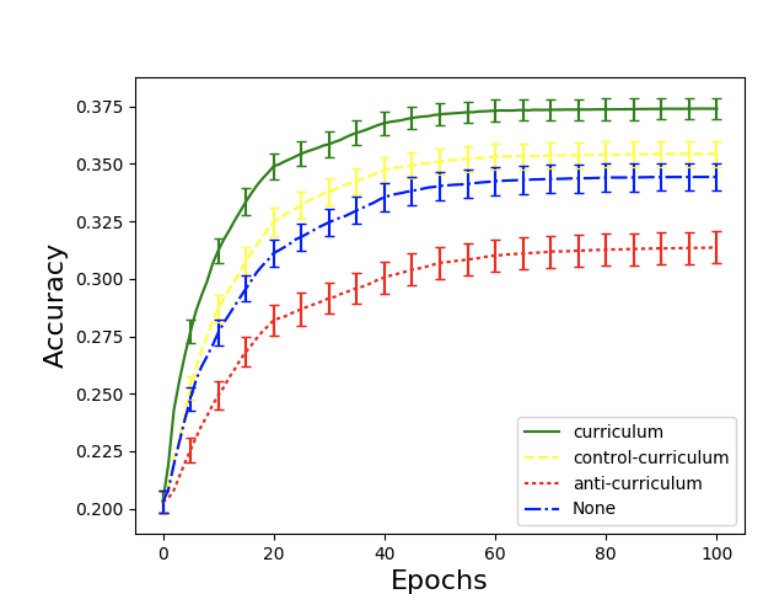
\includegraphics{TransferLearningCurricExample.png}
\caption{Figure 3b from  \cite{weinshall2018curriculum}, test classification accuracy of a convolutional network trained using various curriculum methods on the CIFAR 100 dataset \cite{krizhevsky2009learning}. The curriculum method trains on progressively more difficult samples, while the anti-curriculum method trains on progressively easier samples. The control-curriculum is trained using a random curriculum to control for differences in training between the curriculum methods and the baseline.}
\label{TransferExample}
\end{figure}

A key difficulty in implementing curriculum learning is that it is often very difficult to delineate between `easy' and `difficult' samples, while it is also hard to ascertain how one should transition from different difficulties. A key issue therefore is that of exploring methods for  automating the construction of learning curricula, and it is towards this goal that this paper contributes; specifically investigating how active learning methods can aid such curriculum construction. Having introduced the reader to active and curriculum learning, the next section will lay out a variety of related work wherein the authors attempt to automate the process of curriculum construction or apply active learning methods with the goal of improving network performance. 


\section{Active Learning}\label{Background_ActiveLearning}
A key component in any supervised learning effort is labeled data; in many domains it is relatively easy and cheap to obtain large volumes training samples, however in others it can be far more costly, particularly acquiring accurate labels. In medical image analysis for example one may require a domain expert to spend significant time analysing each image before assigning label, or in document tagging it can take time to read a document and assign a topic label. It can therefore be very useful for a designer to understand which samples they should go to the effort of acquiring, labeling and feeding into their chosen learning algorithm, generally measured by how much the chosen samples improve the network performance, compared to if samples were instead selected randomly. We here introduce some of the main methodologies employed for active learning, giving the reader some background to the methods that will be used in this paper.

There are a variety of approaches to the active learning problem, however most involve the use of an \textit{acquisition function}, which selects which sample, from a set of candidate unlabeled examples, should be selected for labeling and training. As the most appropriate training examples varies depending on the learning algorithm, as well as its current state in the training process, the chosen sample is said to be `queried' by the algorithm. The motivation behind different active learning approaches vary; one of the most common approaches is that of \textit{uncertainty sampling}, wherein the samples that the learning algorithm is most uncertain about labeling are queried. This uncertainty can be captured by analysing the distance to classification threshold of the model outputs; for example one method is to select the sample about which the model is least confident in predicting: (taken from REF SETTLES:)
\begin{equation}
x^{*}_{LC} = \arg\max_{x} 1 - P_{\theta}(\hat{y}|x),
\end{equation}
where
\begin{equation}
\hat{y} = \arg\max_{y}P_{\theta}(y|x).
\end{equation}
Where $x^{*}_{LC}$ is the queried training sample and $P_{\theta}(y_{i}|x)$ is the model's predicted probability that sample $x$ is of class $y_{i}$, given model parameters $\theta$. Similarly, samples can be queried by their average distance to classification threshold or, similarly, the entropy of the algorithm prediction, again taken from REF SETTLES:
\begin{equation}
x^{*}_{H} = \arg\max_{x} - \sum_{i} P_{\theta}(y_i|x)\log P_{\theta}(y_i|x),
\end{equation}
where the sum runs over the possible classes $y_i$.

An alternative approach to querying training samples is to estimate the expected change in model parameters, if trained on a given sample. As, in the active learning setting, it is assumed that the label is unavailable, this is calculated as an average across all potential labels. Model change can be estimated by the magnitude of the gradient vector produced by training on the tuple $\braket{x,y}$. The acquisition function then selects the sample which maximises the expected gradient size (REF SETTLES AGAIN):
\begin{equation}
x^{*}_{EGL} = \arg\max_{x} \sum_{i} P_{\theta}(y_i|x) \norm{\nabla \ell_{\theta}(\mathcal{L} \cup \braket{x,y_{i}})},
\end{equation}
where $\norm{.}$ is the Euclidean norm, $\mathcal{L}$ is the current set of labeled training samples, $\ell$ is the objective function used to train the model and $\nabla \ell_{\theta}(\mathcal{L})$ is the gradient of this objective function with respect to the model parameters $\theta$, when trained on $\mathcal{L}$. This approach therefore finds the sample that leads to the largest expected increase in the gradient when added to the training set $\mathcal{L}$.

Finally, another common approach for active learning is that of \textit{query by committee}; here a population of different models are trained on an initial training set, then the samples about which the models exhibit the most disagreement in their predictions are queried. An example of this is \textit{vote entropy} REF:
\begin{equation}
x_{VE}^{*} = \arg\max_{x} - \sum_{i} \frac{V(y_i)}{C} \log \frac{V(y_i)}{C},
\end{equation}
where $C$ represent the size of the `committee' (i.e. the number of models) and $V(y_i)$ is the number of models in the committee that predict predict label $y_i$. There are obvious parallels here to methods such as ensembling, boosting and bagging, indeed active learning has drawn parallels with several other learning paradigms, such as self-paced learning (REF) and curriculum learning (REF), the latter of which we shall now introduce. 


%Machine Learning x
%Supervised Learning x
%	Overfitting x
%	Train/Val/Test Sets x
%	Generalization Error x
%Deep Learning 
%Convolutional Networks
%Gradient Descent
%Stochastic Gradient Descent
%ADAM
%Curriculum Learning
%	Define
%	Self Paced Learning
%	Diversity
%Active Learning
%Define AADT and BALD active score functions
%Neural Networks - Backpropogation, gradient descent